\section{Química} \label{sec:quimica}

\subsection{Sal de Glauber (\ce{Na2SO4.10H2O})} \label{sec:sal-glauber}

O sulfato de sódio (\ce{Na2SO4}) é um sal inorgânico amplamente empregado na indústria química devido às suas propriedades físico-químicas singulares. Trata-se de um sólido cristalino branco, estável e altamente higroscópico, capaz de atuar como agente dessecante pela formação de seu decahidrato (\ce{Na2SO4 . 10 H2O}), conhecido como sal de Glauber --- a forma hidratada mais comum do composto. Tal sal hidratado foi isolado pela primeira vez no século XVII por Johann Rudolf Glauber, a partir da evaporação de águas minerais ricas em sais sulfatados --- fato que originou seu nome.

A \autoref{fig:glauber-structure} apresenta a estrutura cristalina do composto \ce{Na2SeO4 . 10 H2O}, que é isomórfico ao sal de Glauber (\ce{Na2SO4 . 10 H2O}). Isso significa que ambos compartilham a mesma organização espacial no retículo cristalino, diferindo apenas pela substituição dos átomos de selênio (Se) por enxofre (S). \cite{Kamburov2014}

Na estrutura do \ce{Na2SO4 . 10 H2O}, cada cátion \ce{Na+} encontra-se coordenado a seis moléculas de água, formando unidades octaédricas \ce{[Na(H2O)6]+} (representadas em azul na figura). Além das seis moléculas de água coordenadas a cada \ce{Na+}, há outras quatro moléculas de \ce{H2O} por unidade de fórmula que não estão diretamente ligadas a íons metálicos --- são as chamadas moléculas ``livres''. Essas ocupam os espaços entre as cadeias de \ce{[Na(H2O)6]+} e os ânions tetraédricos \ce{SO4^{2-}} (em amarelo), estabelecendo uma complexa rede tridimensional de ligações de hidrogênio. Cada ânion sulfato participa ativamente dessa rede, interagindo por meio de ligações do tipo \ce{O3S=O\bond{...}H-OH}, tanto com moléculas de água coordenadas quanto com as não coordenadas, formando pontes que interconectam as cadeias octaédricas e estabilizam o retículo cristalino \cite{Kamburov2014}.

\begin{figure}
    \centering
    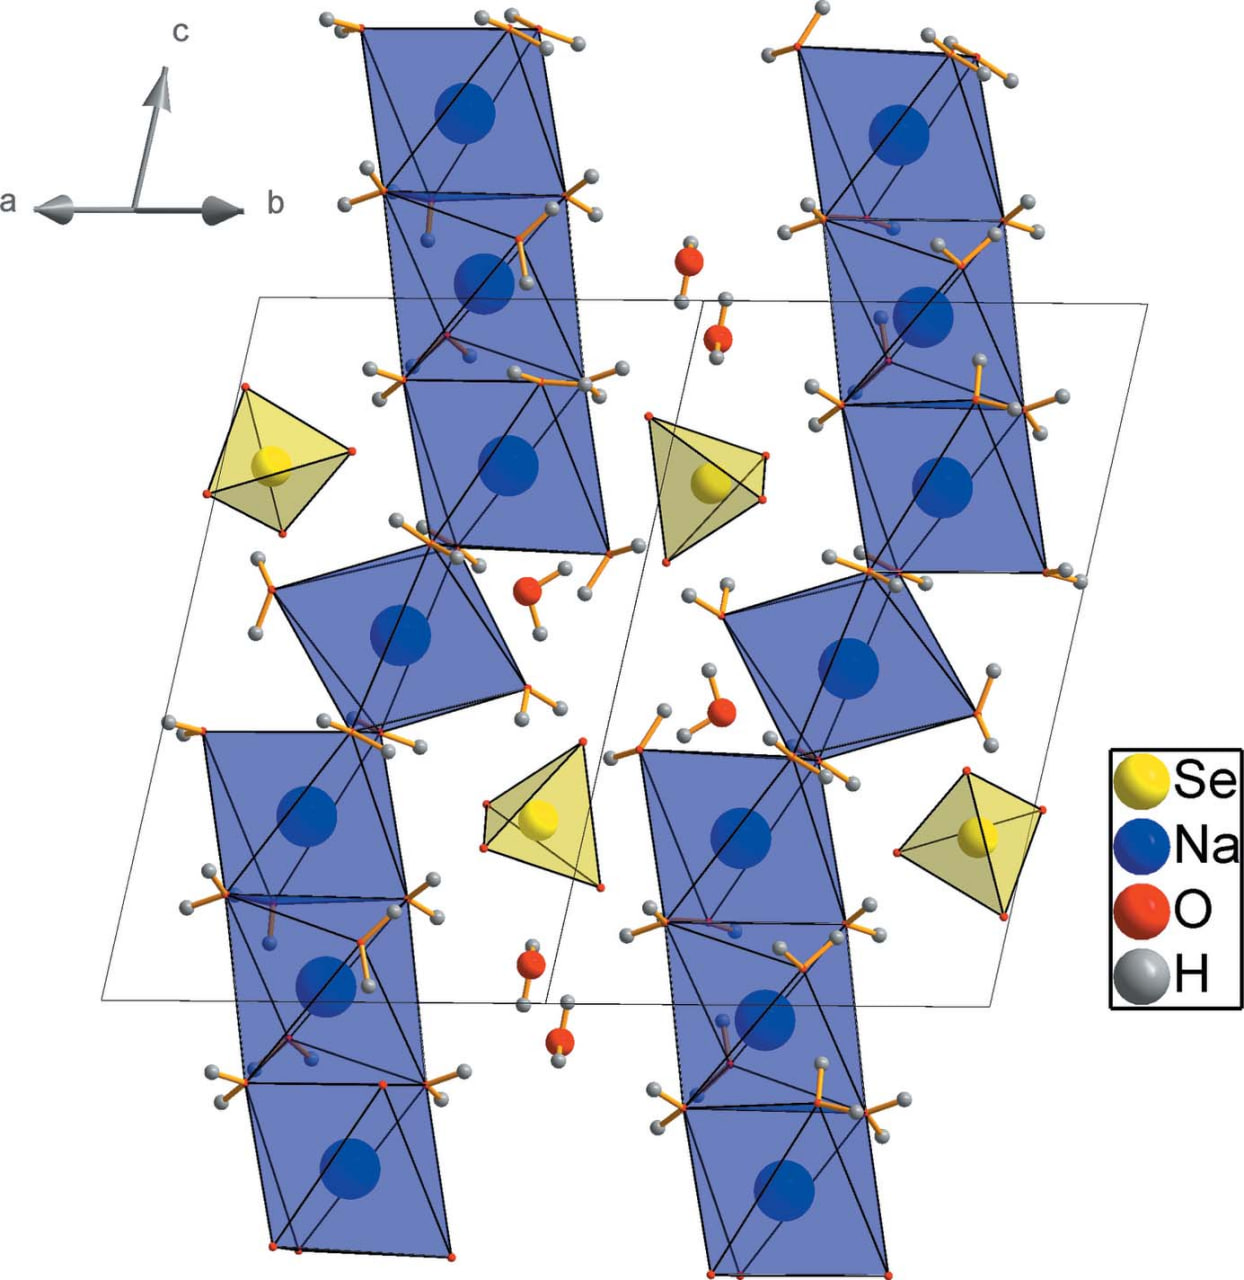
\includegraphics[width=0.4\linewidth]{img/Na2SeO4.10H2O-structure.jpg}
    \caption{Estrutura cristalina do \ce{Na2SeO4 . 10 H2O}, isomorfo ao \ce{Na2SO4 . 10 H2O}. São reportadas 4 unidades de fórmula em cada célula unitária. Fonte: \textcite{Kamburov2014}.}
    \label{fig:glauber-structure}
\end{figure}

É esse arranjo estrutural que permite ao \ce{Na2SO4} incorporar tantas moléculas de água em sua estrutura cristalina (tornando-se \ce{Na2SO4 . 10 H2O}) e, ainda assim, permanecer sólido à temperatura ambiente.
Essa característica enseja a pesquisa e aplicação desse sal em inúmeros processos, como, por exemplo, no controle térmico de painéis fotovoltaicos \cite{Gholami2023}, em sistemas de armazenamento a frio \cite{Xu2018} ou em processos de armazenamento termoquímico \cite{Donkers2015}. Também o efeito de se adicionar outros sais iônicos ao sal de Glauber para modificar suas propriedades tem sido estudado \cite{SankarDeepa2022}.

Para melhor analisar esse tipo de fenômeno, vem à luz as técnicas próprias da análise térmica, especialmente a Análise Termogravimétrica (TGA) e a Calorimetria Exploratória Diferencial (DSC), que submetem a amostra sólida a aquecimento controlado. Essas técnicas são amplamente empregadas na caracterização térmica de materiais: a TGA permite monitorar a variação de massa da amostra em função da temperatura; e a DSC, por sua vez, mostra o fluxo de calor associado aos eventos térmicos (desidratação, no caso em tela). A integração dos picos da DSC também fornece informações sobre a entalpia envolvida no processo --- $\Delta_{\text{desidr.}} H$ neste caso. \cite{Gabbott2008}

\textcite{Rens2012}, a partir das curvas TGA e DSC do sal de Glauber mostradas na \autoref{fig:glauber-tga-dsc}, demonstra que o \ce{Na2SO4 . 10H2O} se decompõe em \ce{Na2SO4} e água líquida a \qty{32}{\celsius}, mediante liberação das moléculas de \ce{H2O} do retículo cristalino, conforme corroborado por \textcite{Donkers2015}.

Analisando a TGA, \textcite{Rens2012} observa que a amostra apresenta uma perda de massa entre \qty{25}{\celsius} e \qty{60}{\celsius}, mas que tal perda de massa é acompanhada por um único pico endotérmico na DSC em $T = \qty{32}{\celsius}$.  O pico único observado na DSC indica que a desidratação propriamente dita ocorre em uma única etapa, \emph{id est}, toda a água quimicamente ligada é liberada em $T = \qty{32}{\celsius}$.

A constante perda de massa observada até os \qty{60}{\celsius} não indica, portanto, nova reação ou decomposição, mas pode ser explicada pela eliminação lenta da água condensada no interior da cápsula de medição, devido à restrição imposta pelo pequeno orifício da tampa, o que retarda sua saída. Esse fato é reforçado pela \autoref{fig:glauber-dsc-water}, que compara a DSC da amostra com a DSC da água pura na mesma configuração experimental. Dessa forma, a desidratação térmica do Sal de Glauber pode ser representada pela \autoref{eq:desidrata-glauber} ou, de forma mais precisa, pela \autoref{eq:desidrata-glauber2}. \cite{Rens2012}%
\begin{equation}%
    \ce{Na2SO4 . 10 H2O (s) <=>[\qty{32}{\celsius}] Na2SO4 (s) + 10 H2O (l)} \label{eq:desidrata-glauber}
\end{equation}%
\begin{equation}%
    \ce{Na2SO4 . 10 H2O (s) + $\Delta_{\text{desidr.}} H$ <=> Na2SO4 (s) + 10 H2O (l)} \label{eq:desidrata-glauber2}
\end{equation}%

\begin{figure}
    \centering
    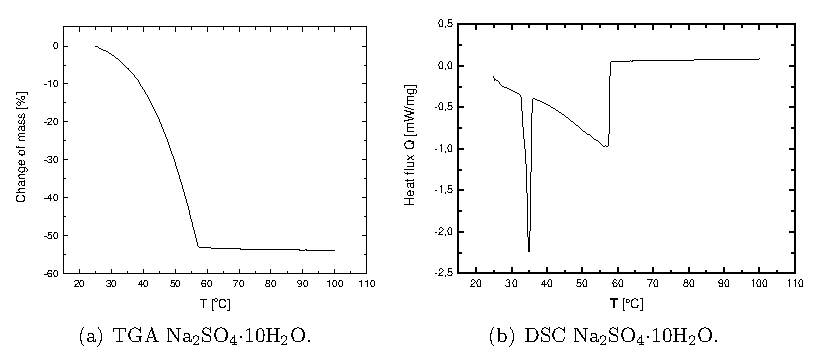
\includegraphics[width=\linewidth]{img/Glauber_TGA_DSC_Rens2012.pdf}
    \caption{Análise TGA e DSC do \ce{Na2SO4 . 10 H2O}, mostrando a desidratação térmica do sal a $T = \qty{32}{\celsius}$. Fonte: \textcite{Rens2012}.}
    \label{fig:glauber-tga-dsc}
\end{figure}

\begin{figure}
    \centering
    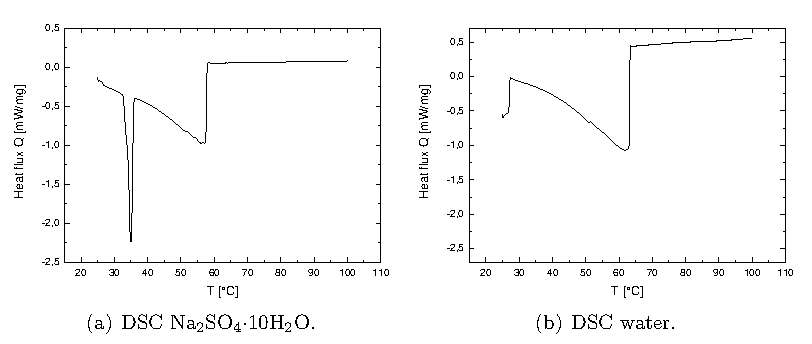
\includegraphics[width=\linewidth]{img/Glauber_Water_DSC_Rens2012.pdf}
    \caption{Análise DSC do \ce{Na2SO4 . 10 H2O} e da água, evidenciando que a perda de massa até $T \leq \qty{60}{\celsius}$ está relacionada à água, e não ao sal. Fonte: \textcite{Rens2012}.}
    \label{fig:glauber-dsc-water}
\end{figure}
